\documentclass{article}

\usepackage{amsmath}
\usepackage{amssymb}
\usepackage{amsfonts}
\usepackage{xcolor}
\usepackage{enumerate}
\usepackage{xeCJK}
\usepackage{physics}

\setCJKmainfont[AutoFakeBold=6,AutoFakeSlant=.4]{Noto Sans CJK SC}
\setCJKmonofont[AutoFakeBold=6,AutoFakeSlant=.4]{Noto Sans CJK SC}

%\setmainfont{URW Gothic L}
%\setmainfont{Century Schoolbook L}
%\setmainfont{Liberation Serif}
%\setmainfont{FreeSerif}

\setlength{\parindent}{0pt} 
\setlength{\parskip}{1em} 

\usepackage[a4paper, total={6in, 9in}]{geometry}

\renewcommand{\labelitemi}{$\bullet$}
\renewcommand{\labelitemii}{$\circ$}
%\renewcommand{\labelitemi}{$\blacksquare$}
%\renewcommand{\labelitemii}{$\box$}
%\renewcommand{\labelitemi}{$\blacktriangleright$}
%\renewcommand{\labelitemii}{$\vartriangleright$}

\usepackage{graphicx}
\graphicspath{ {./} }

\title{SAT Project Report -- OOXX Arrangement Problem}
\author{b07901135 EE3 何國瑋}
\date{2021-05-02}

\begin{document}
    \maketitle

    \section{Problem Definition}


    Given $n$ Xs and $n$ Os that are alternately arranged in $2n$ slots ($n\geq 3$).
    The Goal is to rearrange them with n moves 
    so that all Xs and Os are grouped together respectively.
    2 groups must also be adjacent to each other.

    For example, "$XOXOXO$" has to become "$OOOXXX$" with only 3 moves.

    A Legal move is defined as the following:
    \begin{itemize}
        \item A O/X has to be moved with one of its neighbors.
        \item The two O/Xs can only be moved to two adjacent empty slots.
        \item After they are moved, their original slots become empty.
        \item The total number of slots is unlimited.
    \end{itemize}

    \subsection{Input}
    The Input of the problem is a number n, which represents
    n pairs of "XO" in the begining.

    \subsection{Output}
    The output is a sequence of moves with length n.

    Let $s_k$ denotes the $k^{th}$ slots.
    A move that moves two O/Xs from $s_i$ and $s_{i+1}$ to 
    $s_j$ and $s_{j+1}$ is denoted by
    $$i \rightarrow j$$
        

    \section{SAT Model}

    Although there're solutions for $n=3$, The folloing model only
    focus on solving $n>3$.

    To model this problem, the number of slots is limited to $2n+2$.
    The initial states is the sequence "$XO\dots XOEE$",
    and the final states is the sequence "$EEO\dots OX\dots X$" where E denotes the 
    empty slots.

    Consider a single move between two states, the following variables are defined:
        $$O_0, O_1, \cdots, O_{2n+1}\qquad
        X_0, X_1, \cdots, X_{2n+1}\qquad
        E_0, E_1, \cdots, E_{2n+1}$$
        $$O_0^\prime, O_1^\prime, \cdots, O_{2n+1}^\prime\qquad
        X_0^\prime, X_1^\prime, \cdots, X_{2n+1}^\prime\qquad
        E_0^\prime, E_1^\prime, \cdots, E_{2n+1}^\prime$$
        $$T_0, T_1,\cdots, T_{2n}\qquad Y_0, Y_1$$
    Where
    \begin{itemize}
        \item $O_i$/$X_i$/$E_i$ denotes whether $s_i$ is O/X/Empty before the move.
            Exactly one of these three variables will be true.
        \item $O_i^\prime$/$X_i^\prime$/$E_i^\prime$ denotes whether $s_i$ is O/X/Empty after the move.
            Exactly one of these three variables will be true.
        \item $T_i$ denotes that $s_i$ and $s_{i+1}$ is to be moved.
            Since there's only 2 (adjacent) empyt slots at any time,
            there's only one choice for the destination. 
            Exactly one among all $2n+1$ variables will be true.
        \item $Y_0$ and $Y_1$ denotes whether the two O/Xs to be moved is O or not.
    \end{itemize}

    For $n$ moves, $n+1$ states are needed.  
    Therefore, the variables used in CNF formula includes
    $$O_i^m,X_i^m,E_i^m \qquad 
    \text{$m$ denotes the $m^{th}$ state. \quad$0\leq m < n+1$,\quad$0\leq i < 2n+2$}$$
    $$T_i^m, Y_0^m, Y_1^m \qquad
    \text{$m$ denotes the $m^{th}$ move. \quad$0\leq m < n$,\quad $0\leq i < 2n+1$}$$ 

    \subsection{Basic Constraints}

        \subsubsection{Exactly One}
            
        The "Exactly One" constraints on a set of varaibles
        $\{v_1, v_2,\dots, v_k\}$ are translated to
        $$
        (\Sigma_{i=1}^{k}v_i) \land
        \Pi_{i=1}^{k-1}
        ( \Pi_{j=i+1}^{k} ( \overline v_i \lor \overline v_j ) )$$
        in the CNF formula.

        For each states $m$ and each $i$, exactly one of $\{O^m_i, X^m_i, E^m_i\}$ 
        is true.

        For each move $m$, exactly one of $\{T^m_0, T^m_1, \ldots, T^m_{2n}\}$ is true.
        
        \subsubsection{Initial and Final States}

        The variables $O$, $X$, and $E$ in the initial states 
        and the final state are directly assigned to desired values.

        \subsubsection{Valid Move between 2 States}

        During a move from the $m^{th}$ state to the $m+1^{th}$ state,
        the following terms are constructed to ensure a valid move
        (the superscript $m$ is ignored and the superscript $m+1$ is 
        denoted by $\prime$ for simplicity)

        The term for take rule is
        $$
        \overline T_i \lor 
        (
        \overline E_i
        \overline E_{i+1} 
        E_i^\prime E_{i+1}^\prime
        (\overline Y_0\lor O_i)
        (Y_0\lor X_i)
        (\overline Y_1\lor O_{i+1})
        (Y_1\lor X_{i+1})
        )
        $$
        The term for place rule is
        $$
        \overline T_i^{m-1} \lor 
        (
        E_i E_{i+1} 
        \overline E_i^\prime 
        \overline E_{i+1}^\prime
        (\overline Y_0\lor O_i^\prime)
        (Y_0\lor X_i^\prime)
        (\overline Y_1\lor O_{i+1}^\prime)
        (Y_1\lor X_{i+1}^\prime)
        )
        $$
        And the term for maintaining the value of unmoved slots is
        $$
        T_i^{m-1} \lor
        T_{i-1}^{m-1} \lor
        T_i \lor T_{i-1} \lor
        (\overline O_i\lor O_i^\prime)
        (\overline E_i\lor E_i^\prime)
        (\overline X_i\lor X_i^\prime)
        $$


        The above three terms can be translated to clauses by 
        simply applying distribution law to
        the last product terms.
            
    \subsection{Additional Constraints and Modification}
    \label{added}

    The following constraints and modifications 
    are found by observing the generated solutions.

        \subsubsection{Number of Slots}

        There's always a solution
        when the number of slots is restricted to $2n+2$, 
        Also, with this restriction, the destination of each move has only one choice, 
        so the model can be simplified. 

        \subsubsection{The Second Last State}

        The second last state always looks like the following
        $$XXO\dots OX\dots XEEX$$
        So the last state and the last move is removed from the SAT solver.

        \subsubsection{No Duplicated Moves}

        A move on at slot $s_i$ will happen at most once. 
        That is, among \{$T_i^0, T_i^1, \dots, T_i^{n-2}$\}, at most one variable is true.
        The constraint is translated to
        $$
        \Pi_{m=0}^{n-3}
        ( \Pi_{k=m+1}^{n-2} ( \overline T_i^m \lor \overline T_i^k ) )
        $$

        \subsubsection{The Pattern of the O/X Moved}

        For the first $\lceil n/2\rceil$ moves, the pattern is "$OX, XO, OX,\dots$".\\
        For the last $\lfloor n/2\rfloor$ moves, the pattern is "$\dots, XX, OO, XX$".

        Therefore, the value of $Y_0$ and $Y_1$ in each move can be assigned directly.
            
        \subsubsection{Putting Os and Xs Together}

        Except the first move and the $\lceil (n+1)/2\rceil^{th}$ move, all moves
        take the O/Xs with different neighbors,
        and put them next to correct neighbors.
        So, the following two terms can be added 
        to the take rule and place rule mentioned before.

        $$
        \overline T_i \lor 
        (
        (\overline Y_0\lor X_i)
        (Y_0\lor O_i)
        (\overline Y_1\lor X_{i+1})
        (Y_1\lor O_{i+1})
        )
        $$
        $$
        \overline T_i^{m-1} \lor 
        (
        (\overline Y_0\lor O_{i-1}^\prime)
        (Y_0\lor X_{i-1}^\prime)
        (\overline Y_1\lor O_{i+2}^\prime)
        (Y_1\lor X_{i+2}^\prime)
        )
        $$

    \section{General Solution}

    With the constraints found and the pattern of solutions
    , though didn't expected, a general solution to this
    problem can be derived in linear time.

    First, the sequence is partitioned into the following form (E denotes the empyt slots)
    $$XOXO\quad XOXO\quad \dots\quad OXOX\quad OXOX\quad OEE$$
    For a problem with input size $n=4k+c$, $0\leq c < 4$,

    In the first $2k-1$ moves, alternately perform the following two moves
    \begin{itemize}
        \item Move the "$OX$" in "the left most untouched group" to the empty slots.
        \item Move the "$XO$" in "the right most untouched group" to the empty slots.
    \end{itemize}
    After $2k-1$ moves, the whole sequence will look like this
    $$XXOO\quad XXOO\quad \dots\quad OOXX\quad OOXX\quad OOX$$
    Then, in the middle of the sequence, there're 4 possible cases. For these
    4 cases, apply the following moves 
    (The symbol "$/$" denotes the boundary between Os and Xs at the end)

    For $c=0$, apply 1 move
    $$XEEO\quad XO/X$$
    $$XXOO\quad EE/X$$
    For $c=1$, apply 2 moves
    $$XEEO\quad XOX/O\quad X$$
    $$XXOO\quad XOE/E\quad X$$
    $$XXOE\quad EOO/X\quad X$$
    For $c=2$, apply 3 moves
    $$XEEO\quad XOXO/\quad XOX$$
    $$XXOO\quad EEXO/\quad XOX$$
    $$XXOO\quad OXXO/\quad XEE$$
    $$XXOO\quad OEEO/\quad XXX$$
    For $c=3$, apply 4 moves
    $$XEEO\quad XOXO\quad X/OXO\quad X$$
    $$XXOO\quad XOXO\quad E/EXO\quad X$$
    $$XXOO\quad XEEO\quad O/XXO\quad X$$
    $$XXOO\quad XXOO\quad O/XEE\quad X$$
    $$XXOO\quad EEOO\quad O/XXX\quad X$$

    Finally, after the above moves, there're $k$ pairs of "$XX$" at the LHS of
    the sequence and $k$ pairs of "$OO$" at the RHS of the sequence.

    For the next $2k$ moves, alternately move all the "$OO$" to the left
    and all the "$XX$" to the right. Then the whole process is completed.



    \section{Result of SAT Solver}
        
    The model described at the beginning is actually 
    a version with a few modifications already.
    The original version has more empty slots on both sides
    and have an additional variable $P$ to denote the destination slots.
    In that version, the SAT solver
    can only solve the problem up to $n=16$ within a few minutes.

    After the modifications and improvements mentioned in section \ref{added}, 
    the SAT solver can solve the problem up to $n=150$ in reasonable time.
    before the general solution is found.

    \begin{figure}[h]
        \begin{minipage}{0.99\textwidth}
        \centering
        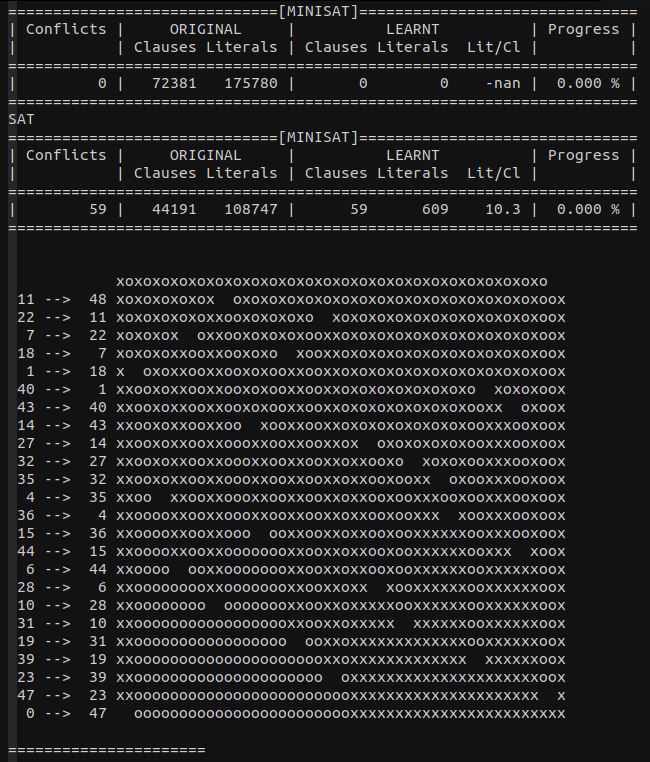
\includegraphics[width=.6\textwidth]{img/24.png}
        \caption{An example output of $n=24$}
        \end{minipage}
    \end{figure}

    The runtime(ticks), number of original clauses, and number of learned clauses
    corresponding is showed in the graph below.

    \begin{figure}[h]
        \begin{minipage}{0.99\textwidth}
        \centering
        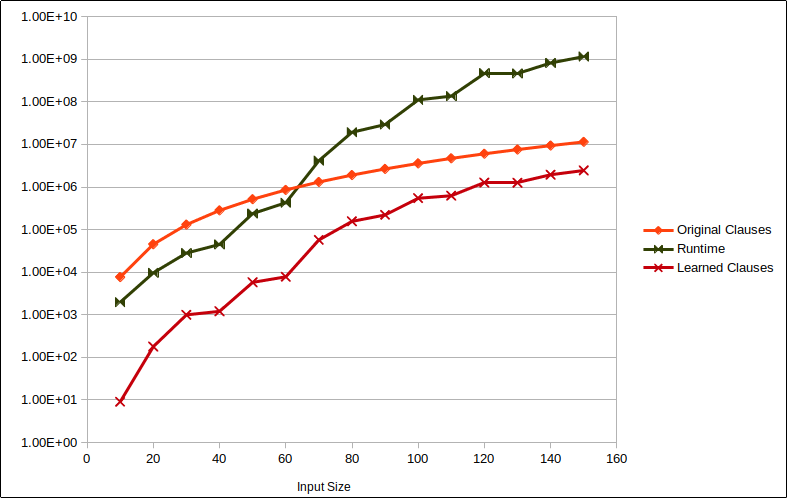
\includegraphics[width=\textwidth]{img/graph.png}
        \caption{Runtime(ticks), number of original clauses, and number of learned clauses versus Input size}
        \label{fig:}
        \end{minipage}
    \end{figure}

    \section{Reference}

    GitHub Link: https://github.com/allen1236/sat-ox-problem 
        


\end{document}
